
\documentclass[10pt,a4paper]{book}
\usepackage{babel}
\usepackage{ctex}
\usepackage[dvipsnames, svgnames, x11names]{xcolor}
\usepackage{amsmath}
\usepackage{amsfonts}
\usepackage{amssymb}%数学符号宏包
\usepackage{geometry}
\usepackage{fancyhdr}
\usepackage{framed}
\usepackage{fontspec}
\usepackage{ntheorem}
\usepackage{nomencl}
\usepackage{nicematrix}
\usepackage{multicol}
\usepackage{indentfirst}%首行缩进
\setlength{\parindent}{2em}
\usepackage[bookmarks=true,colorlinks,linkcolor=black]{hyperref}
\usepackage{CJKfntef}
\usepackage{amsmath,bm}%重要宏包,粗斜体\bm
\usepackage{makeidx}%重要宏包,用于添加索引
\usepackage{pgf,tikz,pgfplots}%一般绘图宏包
\pgfplotsset{compat=1.15}
\usepackage{mathrsfs}
\usetikzlibrary{arrows}
\usepackage{tikz-3dplot}%3d绘图宏包
\usepackage{tcolorbox}%box宏包
\usepackage{subfig}
\usepackage{autobreak}
\usepackage{enumerate}
\usepackage{wasysym}
\usepackage{textcomp}
\usepackage{marginnote}
\usepackage{ulem}%下划线宏包用法和样式如下:
%\uuline{双下划线}
%\uwave{波浪线}
%\sout{中间删除线}
%\xout{斜删除线}
%\dashuline{虚线}
%\dotuline{加点}
\usepackage{titletoc}%目录页的宏包
\usepackage[center]{titlesec}%改变章节或标题的样式的宏包
	\usepackage{pifont} 
	\usepackage[perpage]{footmisc}  %每页脚注重新编号
	\renewcommand{\thefootnote}{\normalsize \ding{\numexpr191+\value{footnote}}}  %使用pifont包里\
\makenomenclature
%\titleformat{command}[shape]{format}{label}{sep}{before}[after]

%1.command 是要重新定义的各种标题命令,比如 \part,\chapter,\section,\subsection,\subsubsection,\paragraph,\subparagraph等;
%2.shape 是用来设定段落形状的,可选的参数有 hang 、 block 、 display 等,详见 titlesec 文档,位于:TEXLIVE/VERSION/texmf-dist/doc/latex/titlesec
%3.format 用于定义标题外观,比如使标题居中、字体加粗等;
%4.label 用于定义定义标题的标签,就是标题内容前面的标号;
%5.sep 定义标题的标签与标题内容之间的间隔距离。
%6.before 用于在标题内容前再加些内容;
%7.after 用于在标题内容后再加些内容。

\usetikzlibrary{shapes,arrows}
\makeindex%添加索引
%缺省页面
\geometry{inner=2cm,outer=2cm,bottom=1.5cm,top=2cm,marginparwidth=3.5cm,marginparsep=0.5cm,includemp}
%\geometry{showframe,showcrop}%此句用于显示排版文本框
%字体设置-------------------------------
\setCJKmainfont[BoldFont={SourceHanSansHC-Medium}]{SourceHanSerifSC-Regular}
\setCJKfamilyfont{song}{SourceHanSerifSC-Regular}
\setCJKfamilyfont{hei}{SourceHanSansHC-Regular}
\setCJKfamilyfont{heiti}{SourceHanSansHC-Medium}
\setCJKfamilyfont{heilight}{SourceHanSansHC-Light}
\setCJKfamilyfont{title}{SourceHanSansHC-Regular}
\setCJKfamilyfont{songbold}{SourceHanSerifSC-SemiBold}
\theorembodyfont{\CJKfamily{song}}
%\setmainfont{Times New Roman}
%颜色设置-——————————
\definecolor{f8766d}{HTML}{EA7500}
\definecolor{1a9850}{HTML}{0097e6}
\definecolor{ffa725}{HTML}{1289A7}
\definecolor{2a7ae2}{HTML}{7158e2}
\definecolor{6a3d9a}{HTML}{ED4C67}
\definecolor{53a9ab}{HTML}{007500}
\definecolor{titlepurple}{HTML}{5758BB}
\definecolor{titlepurpleb}{HTML}{833471}
\definecolor{titlepurplec}{HTML}{006266}
\definecolor{md}{HTML}{EA2027}
\definecolor{background}{HTML}{f5f5ed}
%geogebra颜色
\definecolor{zzttqq}{rgb}{0.6,0.2,0}
\definecolor{uuuuuu}{rgb}{0.26666666666666666,0.26666666666666666,0.26666666666666666}
\definecolor{ududff}{rgb}{0.30196078431372547,0.30196078431372547,1}
\definecolor{xdxdff}{rgb}{0.49019607843137253,0.49019607843137253,1}
%定理定义环境设置--------------------

%\newtcbox{\mybox}[1][]{on line,
%	arc=0pt,outer arc=0pt,colback=#1!10!white,colframe=#1,
%	boxsep=0pt,left=3pt,right=3pt,top=2pt,bottom=2pt,
%	boxrule=0pt,leftrule=1.5pt}

\newcommand{\mybox}[2][]{
	\begin{tcolorbox}[on line,
		arc=0pt,outer arc=0pt,colback=#1!7!white,colframe=#1,
		boxsep=0pt,left=3pt,right=3pt,top=3pt,bottom=3pt,
		boxrule=0pt,leftrule=1.5pt]#2
\end{tcolorbox}}

\newcounter{A}[section]
\newcounter{B}[section]
\newcounter{C}[section]
\newcounter{D}[section]
\newcounter{E}[section]
\newcounter{F}[section]

\newcommand{\con}[1]{{\bfseries\refstepcounter{#1}\thesection.\arabic{#1}}}

%\theoremindent0.2cm
%\theoremheaderfont{\CJKfamily{songbold}}
%\theoremstyle{break}

%\newtheorem*{theorem}{\hspace{-0.16cm}\color{2a7ae2}\mybox[2a7ae2]{\color{2a7ae2}定理\addtocounter{A}{1} \thesection.\arabic{A}}}
%\newtheorem*{definition}{\hspace{-0.16cm}\color{f8766d}\mybox[f8766d]{\color{f8766d}定义\addtocounter{B}{1} \thesection.\arabic{B}}}
%\newtheorem*{feature}{\hspace{-0.16cm}\color{ffa725}\mybox[ffa725]{\color{ffa725}性质\addtocounter{C}{1} \thesection.\arabic{C}}}
%\newtheorem*{inference}{\hspace{-0.16cm}\color{1a9850}\mybox[1a9850]{\color{1a9850}推论\addtocounter{D}{1} \thesection.\arabic{D}}}
%\newtheorem*{method}{\hspace{-0.16cm}\color{6a3d9a}\mybox[6a3d9a]{\color{6a3d9a}方法\addtocounter{E}{1} \thesection.\arabic{E}}}
%\newtheorem*{example}{\hspace{-0.16cm}\color{53a9ab}\mybox[53a9ab]{\color{53a9ab}例题\addtocounter{F}{1} \thesection.\arabic{F}}}

\newcommand{\theorem}[1][]{\vspace{0.5em}\par\noindent\hspace{-8pt}\mybox[2a7ae2]{\color{2a7ae2}{\CJKfamily{heiti}定理\ \con{A}\hspace{1em}{\CJKfamily{songbold}#1} } }\vspace{0.1em}\par }
\newcommand{\definition}[1][]{\vspace{0.5em}\par\noindent\hspace{-8pt}\mybox[53a9ab]{\color{53a9ab}{\CJKfamily{heiti}定义\ \con{B}\hspace{1em}{\CJKfamily{songbold}#1} } }\vspace{0.1em}\par }
\newcommand{\feature}[1][]{\vspace{0.5em}\par\noindent\hspace{-8pt}\mybox[ffa725]{\color{ffa725}{\CJKfamily{heiti}性质\ \con{C}\hspace{1em}{\CJKfamily{songbold}#1} } }\vspace{0.1em}\par }
\newcommand{\inference}[1][]{\vspace{0.5em}\par\noindent\hspace{-8pt}\mybox[1a9850]{\color{1a9850}{\CJKfamily{heiti}推论\ \con{D}\hspace{1em}{\CJKfamily{songbold}#1} } }\vspace{0.1em}\par }
\newcommand{\method}[1][]{\vspace{0.5em}\par\noindent\hspace{-8pt}\mybox[6a3d9a]{\color{6a3d9a}{\CJKfamily{heiti}方法\ \con{E}\hspace{1em}{\CJKfamily{songbold}#1} } }\vspace{0.1em}\par }
\newcommand{\example}[1][]{\vspace{0.5em}\par\noindent\hspace{-8pt}\mybox[f8766d]{\color{f8766d}{\CJKfamily{heiti}例题\ \con{F}\hspace{1em}{\CJKfamily{songbold}#1} } }\vspace{0.1em}\par }

%符号设置-------------------------------
{\color{titlepurple}}
%标题配置—————————————
\title{
	\begin{center}
		\includegraphics[width=16cm]{covertitle.eps}
		%\includegraphics[width=8cm]{cover2.png}
		%\includegraphics[width=8cm]{cover3.png}
		%\includegraphics[width=12cm]{cover4.png}
	\end{center}
	\vspace{5cm}}
\author{\large\color{titlepurple}关舒文\\{\color{titlepurple}\kaishu{华南理工大学}}}
\date{\color{titlepurple}\small{Latest Update\ :\ \today}}

%章节或标题的样式-------------------
\titleformat{\chapter}{\CJKfamily{title}\huge\color{titlepurple}}{\includegraphics[height=2cm]{sigmaformal.eps} 第\ \thechapter\ 章\ }{0pt}{}
\titleformat{\section}{\CJKfamily{hei}\large\color{titlepurpleb}}{\bfseries{\thesection}\quad  }{0pt}{}
\titleformat{\subsection}{\CJKfamily{hei}\large\color{titlepurplec}}{\bfseries{\thesubsection}\quad  }{0pt}{}
\titleformat{\subsubsection}{\CJKfamily{hei}\normalsize\color{titlepurplec}}{\bfseries{\thesubsubsection}\quad  }{0pt}{}
\renewcommand{\nomname}{符号说明}
%自定义优化命令-----------------------
\renewcommand{\a}{\ensuremath A}%
\renewcommand{\b}{\ensuremath B}%
\renewcommand{\c}{\ensuremath C}%
\renewcommand{\o}{\ensuremath \varnothing}%
\renewcommand{\textbf}[1]{{\CJKfamily{heiti}#1}}%
\newcommand{\md}[1]{{\,\color{purple}#1\,}}%
\newcommand{\cf}[1]{\textit{cf.Fig~\ref{#1}}}%
\newcommand{\margin}[1]{{\marginpar{\footnotesize\kaishu\hspace*{2em}#1}}}
%\renewcommand{\chapter}[1]{{\chapter{#1}\thispagestyle{empty}} }%
%使用了自定义页眉页脚---------------
\pagestyle{fancy}
\renewcommand{\chaptermark}[1]{\markboth{\;第\ \thechapter\ 章\quad#1\;}{}}
\renewcommand{\sectionmark}[1]{\markright{\;\thesection\ #1\;}}
\fancyhf{}
%\fancyfoot[C]{\bfseries\thepage}
\fancyhead[LO]{\small\CJKfamily{heilight}\rightmark}
\fancyhead[RE]{\small\CJKfamily{heilight}\leftmark}
\fancyhead[RO,LE]{\;\thepage\;}
\fancyfoot[RO,LE]{\small\CJKfamily{heilight}{概率论\&数理统计}}
\fancyfoot[RE,LO]{\small\CJKfamily{heilight}Probability and Mathematical Statistics}
\renewcommand{\headrulewidth}{0.4pt} % 注意不用\setlength
%\renewcommand{\footrulewidth}{0pt}
\fancyheadoffset[LE,RO]{4cm}
\fancyfootoffset[LE,RO]{4cm}
%正文部分—————————————
\begin{document}


%目录与公式编号生成——————————
\numberwithin{equation}{section}
\allowdisplaybreaks%强制自动换行
\newgeometry{left=2cm,right=2cm,marginparwidth=0cm,marginparsep=0cm}%封面设置
\pagenumbering{roman}
\maketitle
\thispagestyle{empty}
%页面重新配置----------------------------
\restoregeometry
{\printnomenclature
    \setcounter{page}{0}\pagenumbering{roman}
    \addcontentsline{toc}{chapter}{符号说明}}
\newpage
\pagenumbering{Roman}
\setcounter{page}{0}
\tableofcontents
%色块--------------------------------------
\nomenclature{\colorbox{f8766d}{\qquad} }{Color \texttt{\#EA7500}}
\nomenclature{\colorbox{1a9850}{\qquad}}{Color \texttt{\#0097e6}}
\nomenclature{\colorbox{ffa725}{\qquad}}{Color \texttt{\#1289A7}}
\nomenclature{\colorbox{2a7ae2}{\qquad} }{Color \texttt{\#7158e2}}
\nomenclature{\colorbox{6a3d9a}{\qquad}}{Color \texttt{\#ED4C67}}
\nomenclature{\colorbox{53a9ab}{\qquad}}{Color \texttt{\#007500}}
\nomenclature{\colorbox{titlepurple}{\qquad }}{Color \texttt{\#5758BB}}
\nomenclature{\colorbox{titlepurpleb}{\qquad}}{Color \texttt{\#833471}}
\nomenclature{\colorbox{titlepurplec}{\qquad}}{Color \texttt{\#006266}}
\nomenclature{\colorbox{md}{\qquad}}{Color \texttt{\#EA2027}}
\nomenclature{\colorbox{purple}{\qquad}}{Color \texttt{\#bf0040}}
%正文开始—————————————---------------------------------------------------------------------------------------可以使用\boldmath输入粗斜体与\unboldmath合用
\chapter{概率论的基本概念}
\pagenumbering{arabic}
\setcounter{page}{1}
\definition[概率论研究的对象]
\begin{enumerate}
    \item \textbf{确定性现象} \quad 满足一定条件时,该类现象的结果可以预见(并不一定所有内容都可预测,结果部分具有确定性,部分具有偶然性);
    \item \textbf{偶然性现象}\quad  结果无法预见的现象(部分现象可研究,部分现象仍是临界问题,目前无法研究,但可以找到其特征);
    \item\textbf{ 随机现象}\quad  一部分偶然性现象可以在基本相同的条件下\md{重复观测或重复试验},并且随着\md{观测或试验次数的增多},不同结果的出现次数呈现出\textbf{统计规律}.
\end{enumerate}

在大量的重复试验或观察中所呈现的固有规律性,称为\textbf{统计规律性}. \index{TJGLX@统计概率性}\textbf{概率论是研究随机现象的统计规律的科学}.

\begin{inference}[随机现象的判别标准]
    通过判断事件是否可以在基本相同的条件下重复观测或重复试验,并且随着观测或试验次数的增多,不同结果的是否会出现次数呈现出统计规律.
\end{inference}
\definition[概率论的特点]
\begin{itemize}
    \item 用确定的数学去研究随机现象;
    \item 研究非确定的现象:用于数理金融,控制论,寿险精算,统计物理学等,{ 由于科技手段的限制,或者经济成本的考量,很多事件适合从随机角度去研究} ;
    \item 以确定的数学为工具:排列组合,微积分,线性代数等,{ 本质上是要利用\md{数学工具}来量化这种非确定性的程度}.
\end{itemize}

\begin{example}
    甲、乙两人赌技相同,各出赌注300元。约定:谁先胜三局,则拿走全部600元。现已赌了三局,甲二胜一负,因故要中止赌博,问这600 元要如何分才算公平?
    \begin{enumerate}[\textbf{解法} 1:]
        \item 以已经获胜的局数作为分赌注的依据 甲:$ 600×2/3 = 400 $, 乙:$ 600×1/3 = 200 $. \\存在问题:不具有可扩展性,若只赌一盘,.则不公平.
        \item 设想继续赌下去,甲,乙获胜的可能性分别是多大,以此作为分赌注的依据. 最多还需要两局,结果为四种情况:甲甲,甲乙,乙甲,乙乙.由于甲乙赌技相同,这四种情况出现的可能性相等.前三种情况下甲最终获胜.因此甲,乙最终获胜的可能性大小为$ 3:1 $,即甲分得$ 450 $元,乙分得$ 150 $ 元. \\
              推广:将这一分配方案进行扩展.假设只赌了1局并且甲获胜,该如何分配?\\
              将4局全部比完,可罗列出以下情形 \cf{fig1}:
              \begin{figure}[htbp]
                  \centering
                  \includegraphics[width=\textwidth]{1.1.eps}
                  \caption{可能发生的情形}\label{fig1}
              \end{figure}
    \end{enumerate}
\end{example}
\definition
\begin{itemize}
    \item 概率论(实践):对随机现象有基本认知的前提下,进行演绎推理;
    \item 数理统计(理论):试图通过试验来认知随机现象,处理问题的思路往往来自概率论的有关结果.
\end{itemize}

\section{随机现象与随机试验}
\definition[随机试验]
对随机现象的一次观测或实际实验,统称为\textbf{随机试验},其具有以下特点(判断依据):
\begin{enumerate}
    \item 可以在相同的条件下重复进行;
    \item 每次实验的可能结果不止一个,并且能够事先明确实验的所有可能结果;
    \item 进行一次试验之前不能确定哪一个结果会出现.
\end{enumerate}

\section{样本空间,随机事件}
\subsection{样本空间}
\definition[样本空间]
我们将随机试验$ E $的\md{所有可能结果}组成的集合称为$ E $的\textbf{样本空间}\index{YBKJ@样本空间},记为$ S $.其中样本空间的元素,即$ E $的每个结果,称为样本点\index{YBD@样本点}.

\subsection{随机事件}
\definition[随机事件]\label{sjsj}
试验$ E $的样本空间$ S $的子集为$ E $的\textbf{随机事件}或称\textbf{事件}\footnote{严格地说,事件是指$ S $中满足某些条件的子集当且仅当$ S $是由有限个元素或由可列无限个元素组成的,每个子集才可以看作一个事件.}\index{SJSJ@随机事件}.在每次实验中,当且仅当这一中的样本点出现时,称这一\textbf{事件发生}. \index{SJFS@事件发生}

特别地,有一个样本点组成的\md{单点集},称为\textbf{基本事件}. \index{JBSJ@基本事件}

\definition
对于样本空间$ S $,其包含的所有样本点即$ S $是样本空间的全集,也为其最大的子集.空集$ \varnothing $不包含任何样本点,它也作为样本空间的子集.根据事件的定义\ref{sjsj}:
\begin{itemize}
    \item $ S $称为\textbf{必然事件};\index{BRSJ@必然事件}
    \item$ \varnothing $称为\textbf{不可能事件}. \index{BKNSJ@不可能事件}
\end{itemize}

\subsection{事件间的关系与事件的运算}

事件是一个集合,事件间的关系与运算自然需要并遵循集合论.下面我们根据`` 事件发生的含义'' 以及集合的关系与运算,给出他们在概率论中的定义:
\definition

\margin{ \vspace{2em}\par \hspace*{2em}左图可以直观地表示上述各种关系.长方形所围绕的空间为\md{样本空间$ S $},圆\a 与圆\b 分别表示事件\a 于事件\b,阴影表示\md{事件与事件间}以及\md{事件与样本空间}间的关系.}
\begin{figure}[htbp]
    \centering
    \subfloat[]{\label{sub-fig-1}
        \begin{minipage}{0.33\textwidth}
            \centering
            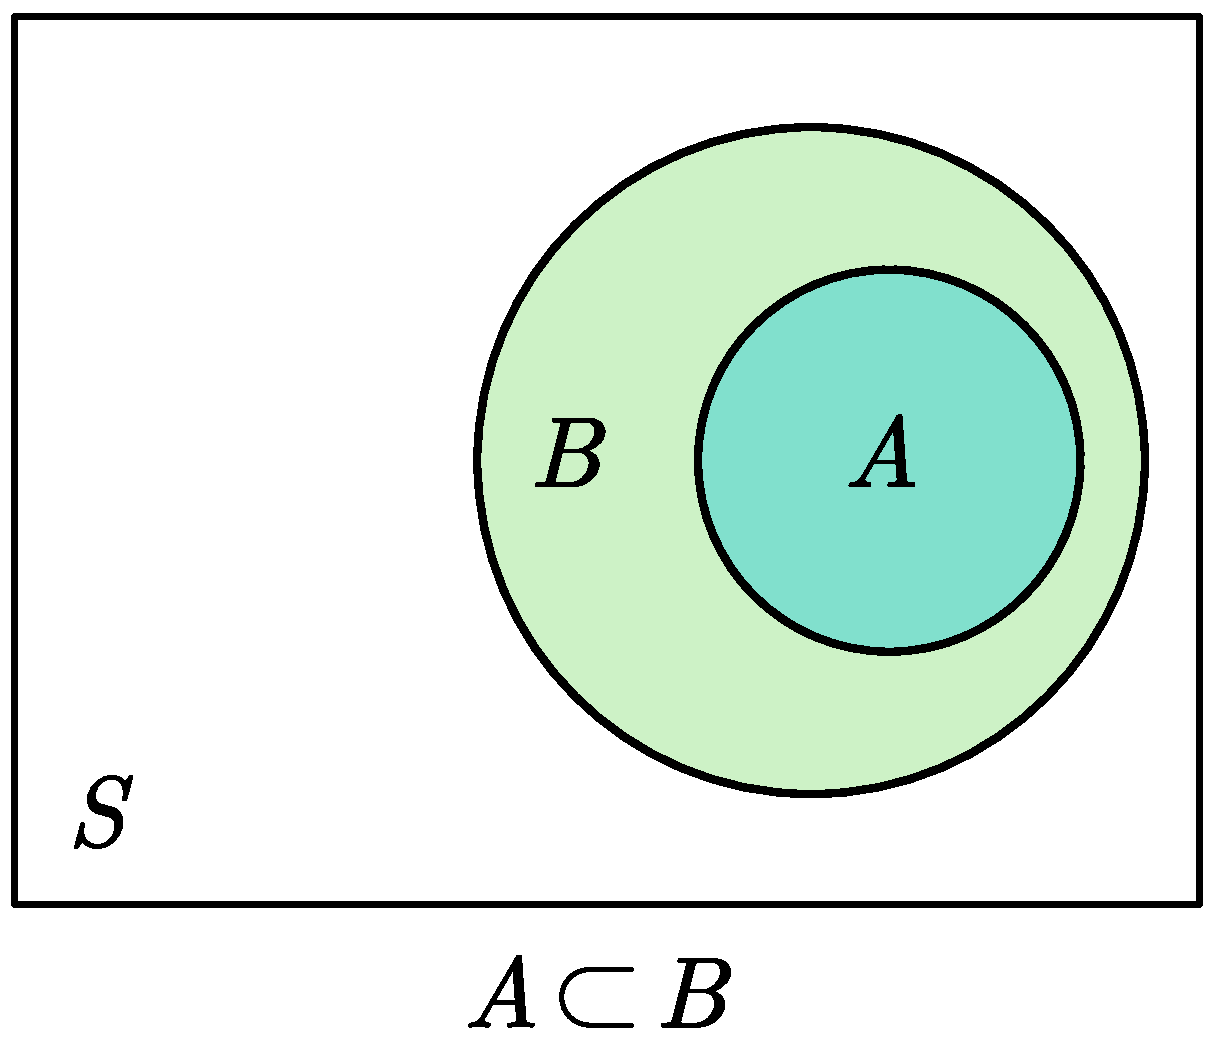
\includegraphics[width=0.8\linewidth]{sj1.pdf}
        \end{minipage}}
    \subfloat[]{\label{sub-fig-2}
        \begin{minipage}{0.33\textwidth}
            \centering
            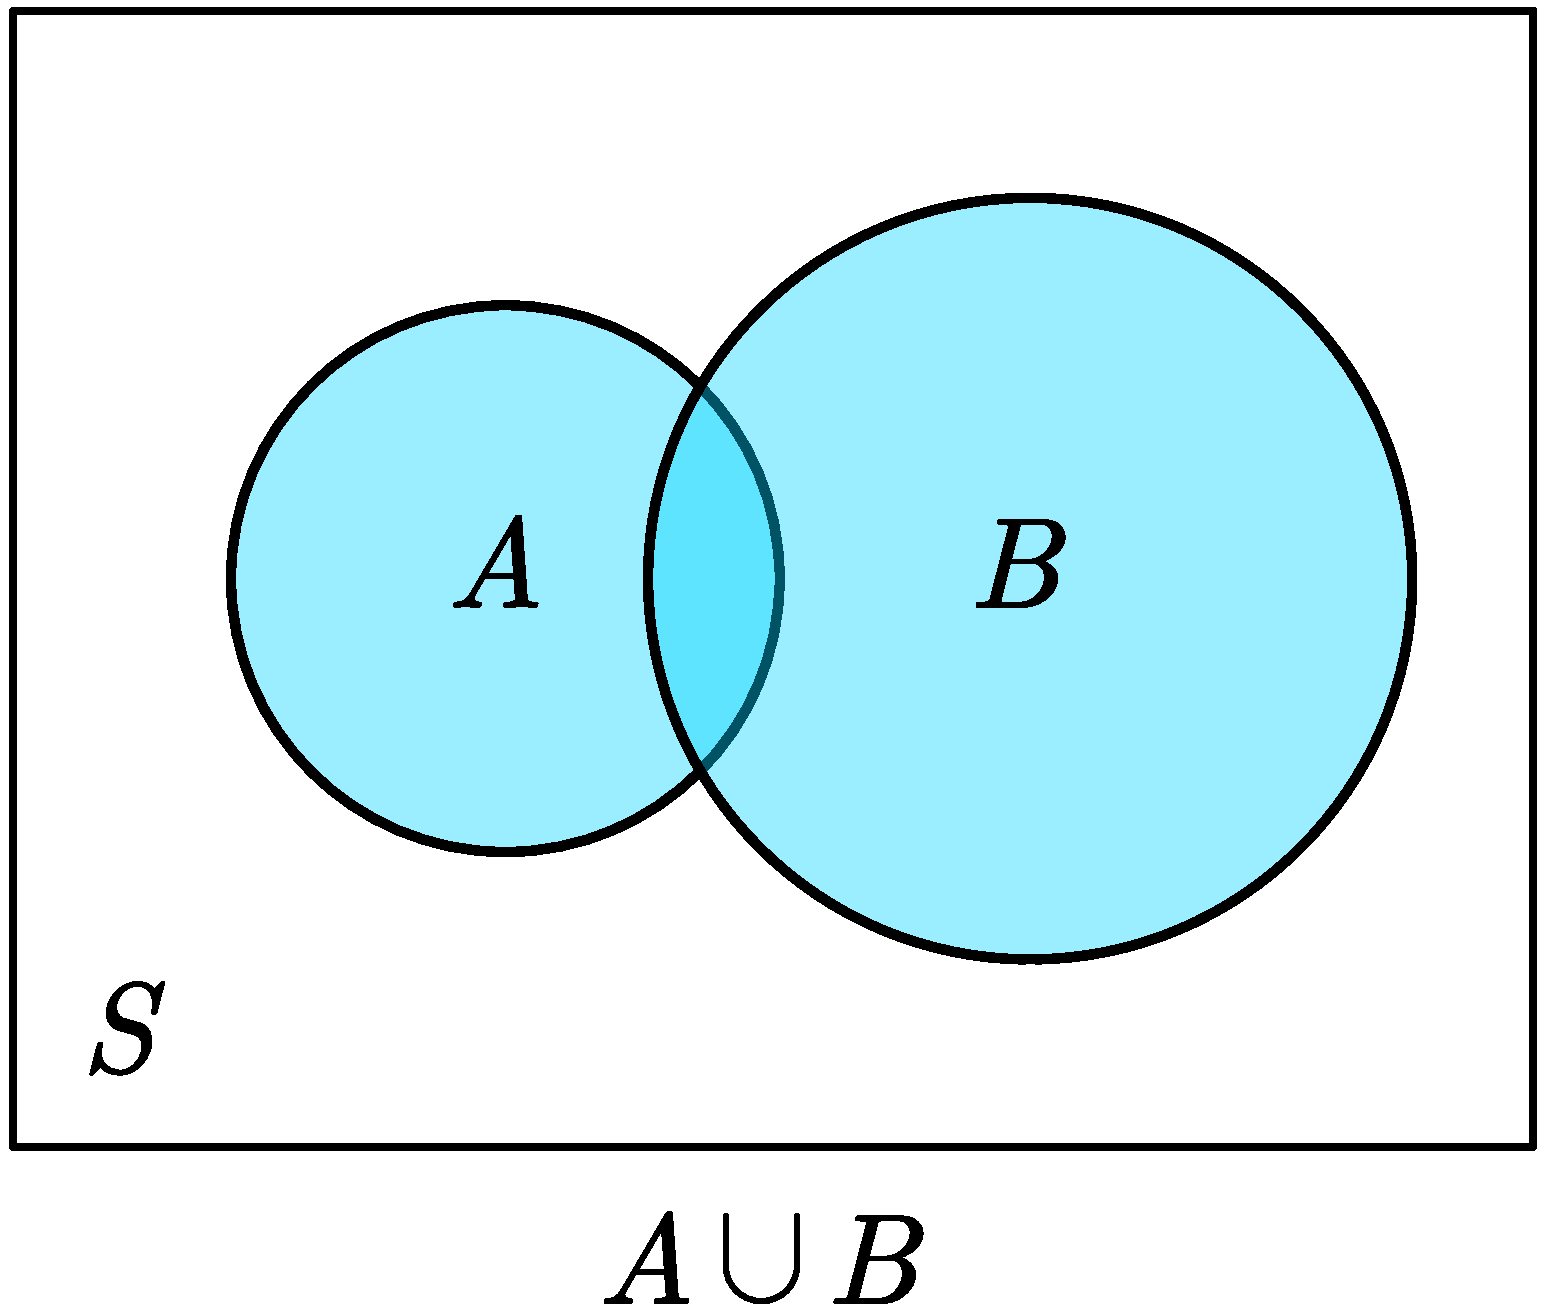
\includegraphics[width=0.8\linewidth]{sj2.pdf}
        \end{minipage}}
    \subfloat[]{\label{sub-fig-3}
        \begin{minipage}{0.33\textwidth}
            \centering
            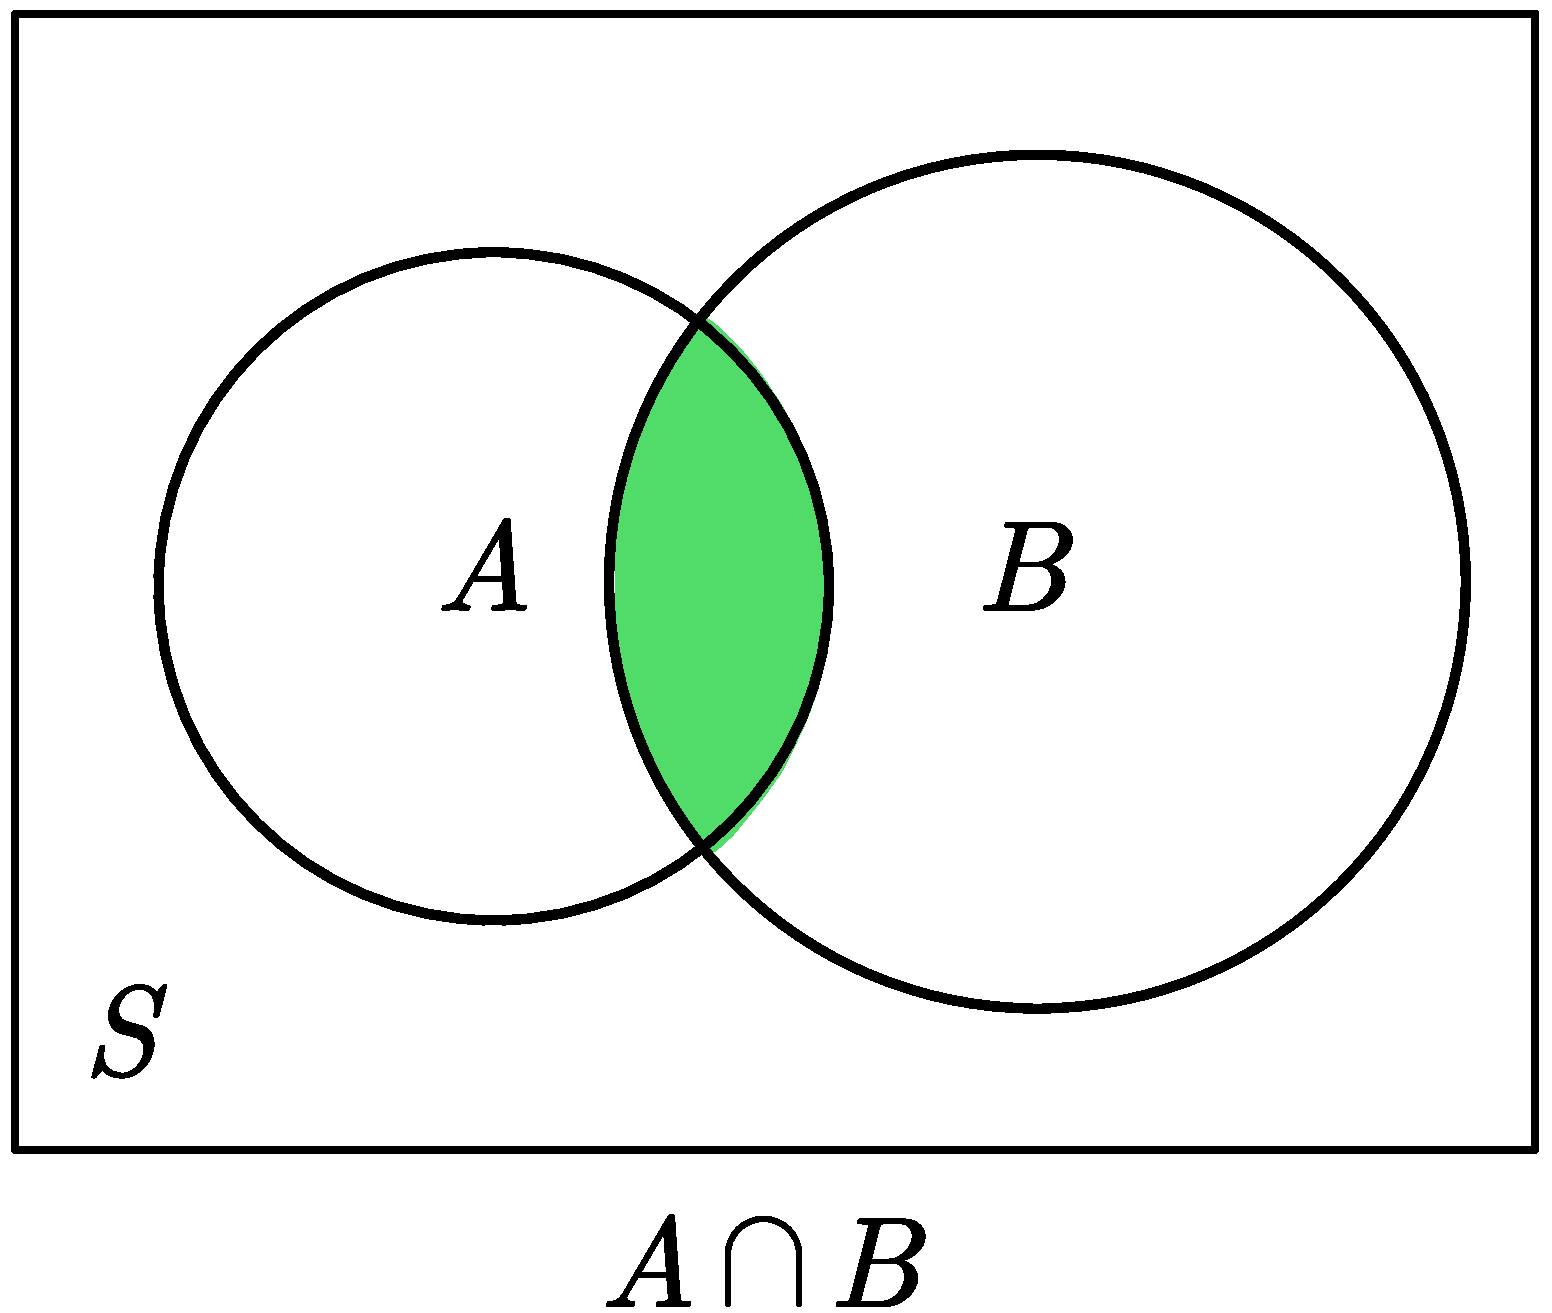
\includegraphics[width=0.8\linewidth]{sj3.pdf}
        \end{minipage}}\\
    \subfloat[]{\label{sub-fig-4}
        \begin{minipage}{0.33\textwidth}
            \centering
            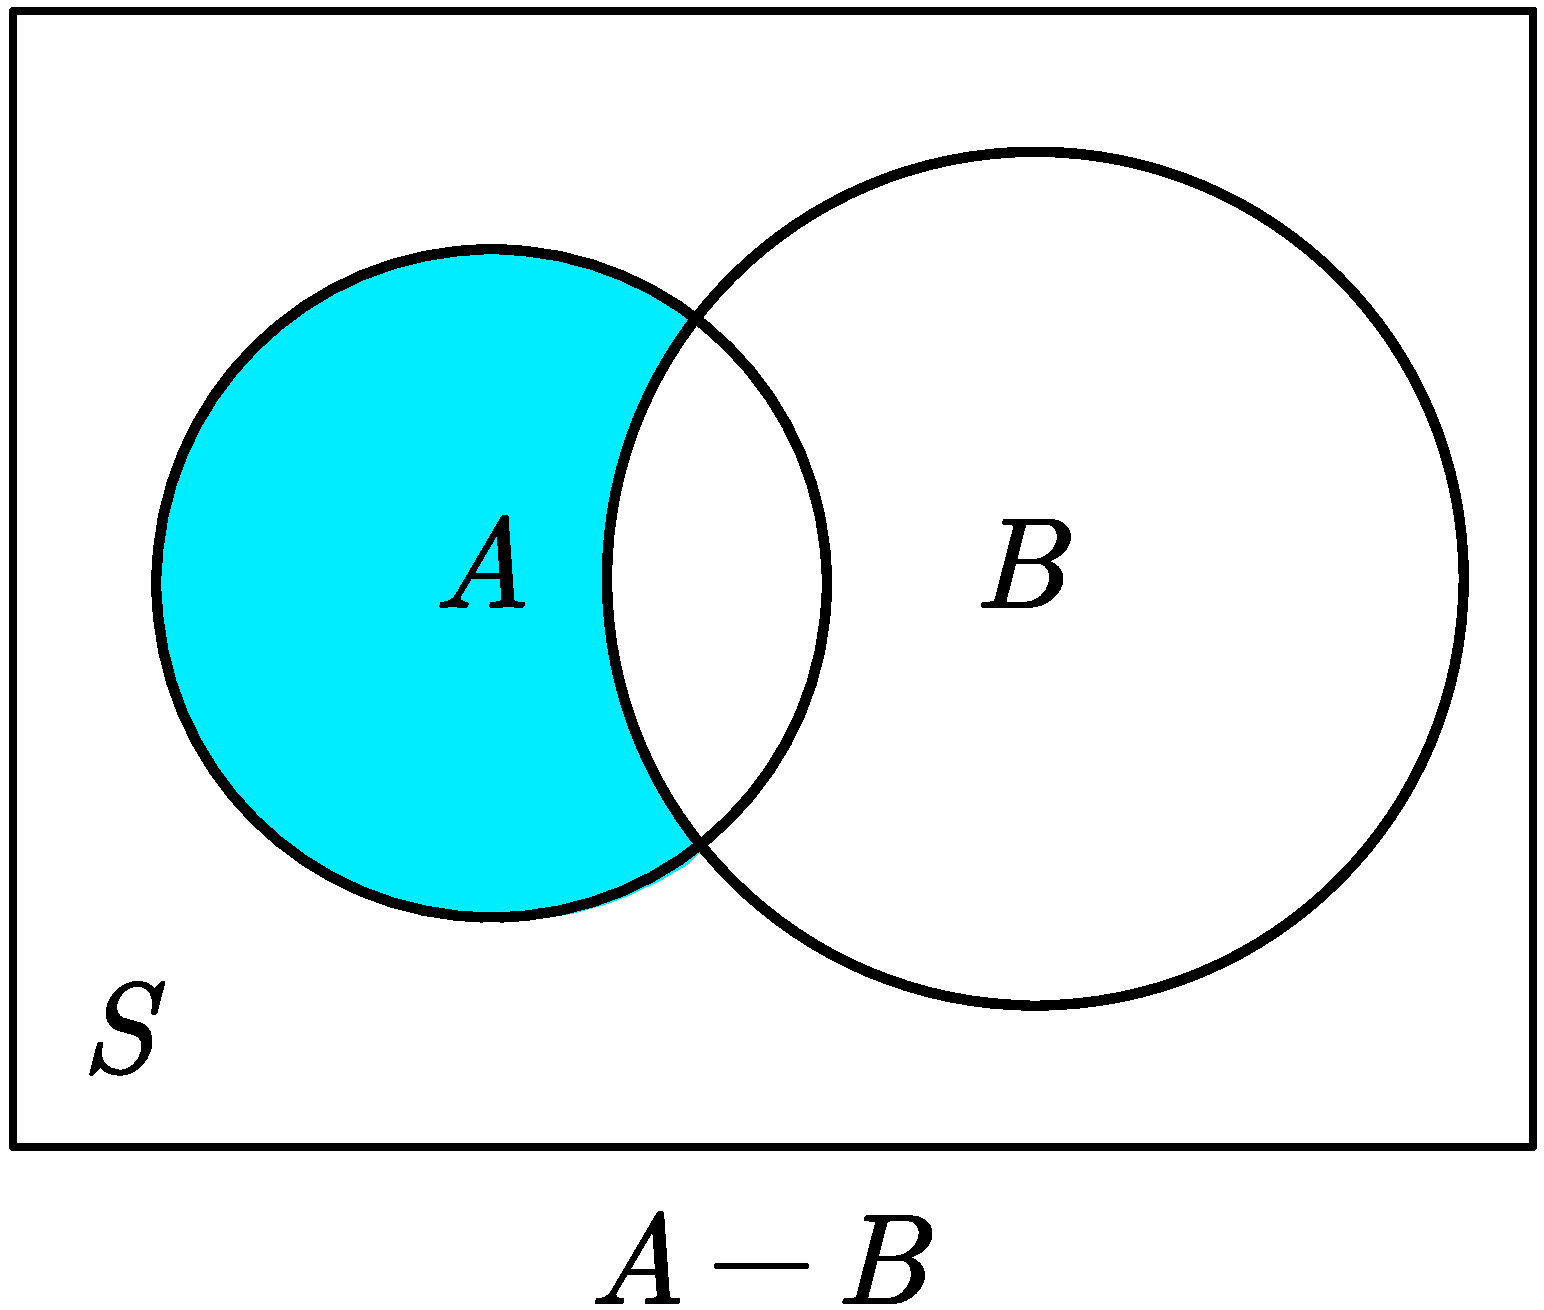
\includegraphics[width=0.8\linewidth]{sj4.pdf}
        \end{minipage}}
    \subfloat[]{\label{sub-fig-5}
        \begin{minipage}{0.33\textwidth}
            \centering
            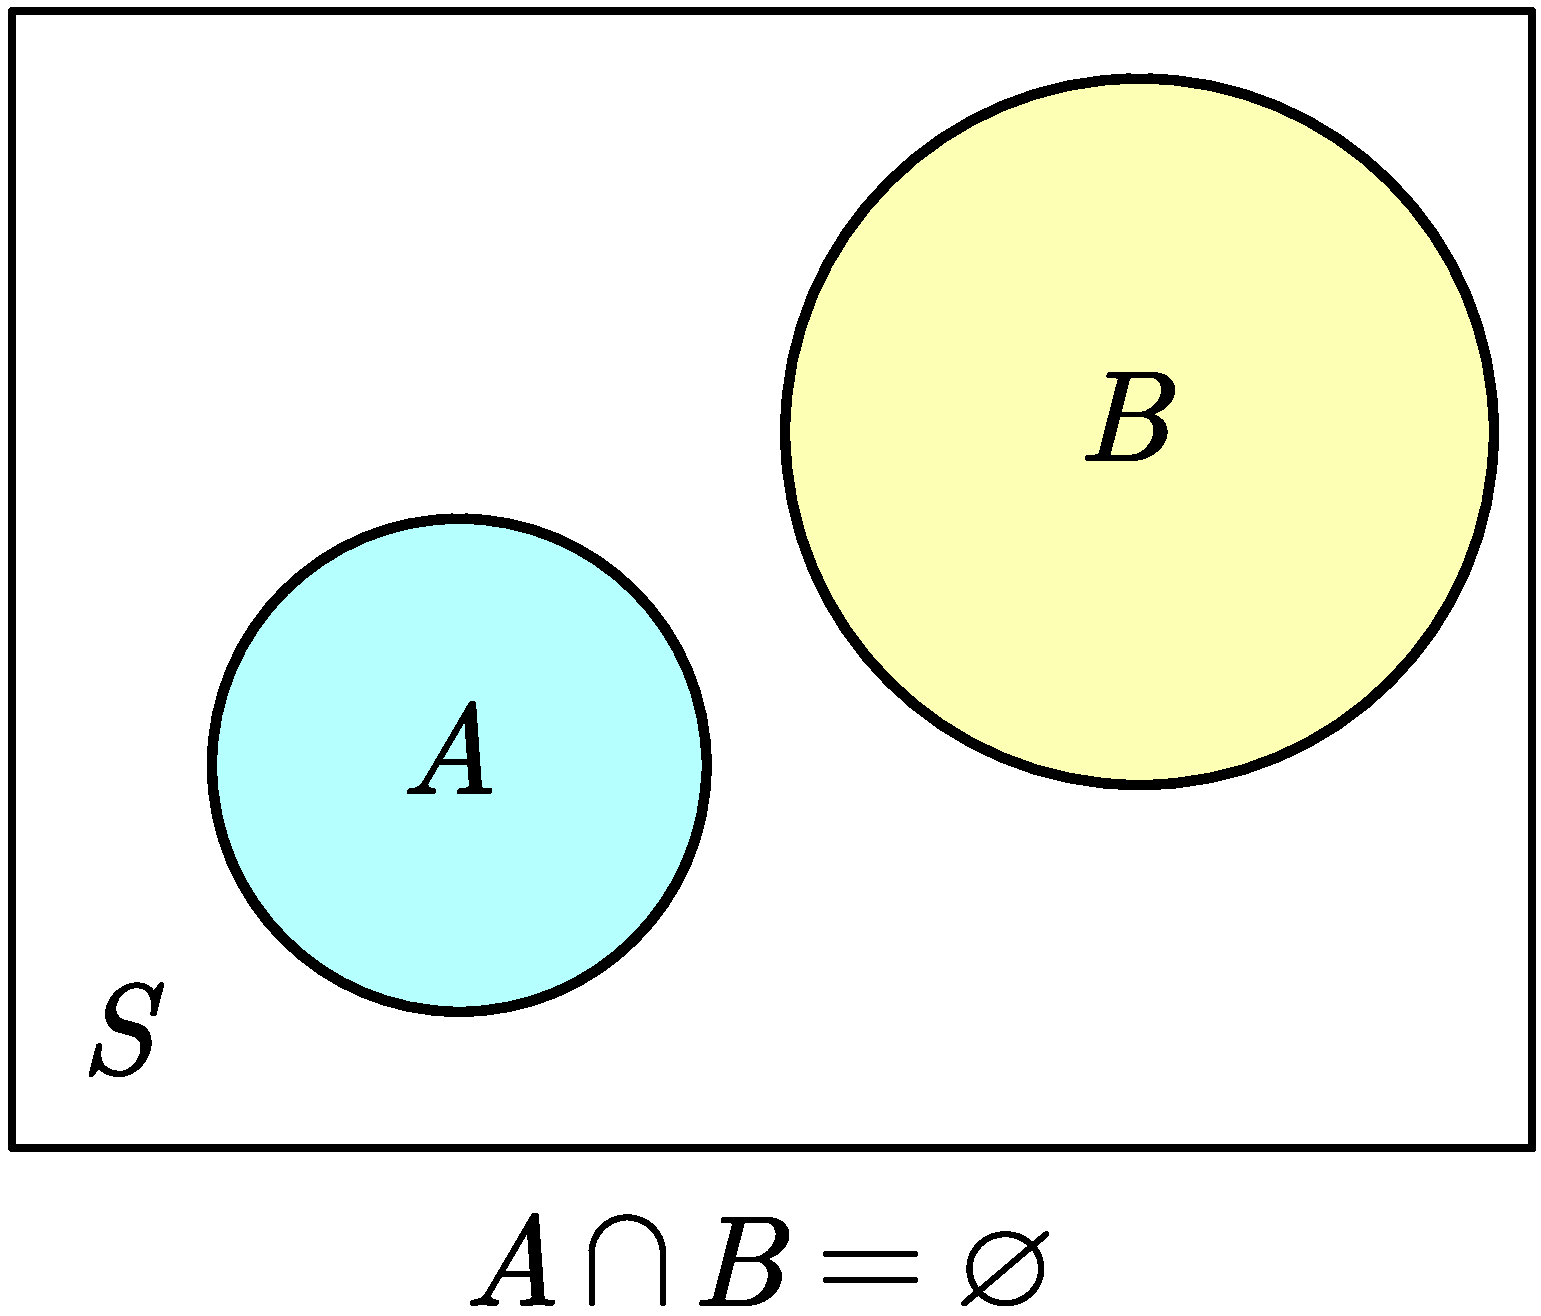
\includegraphics[width=0.8\linewidth]{sj5.pdf}
        \end{minipage}}
    \subfloat[]{\label{sub-fig-6}
        \begin{minipage}{0.33\textwidth}
            \centering
            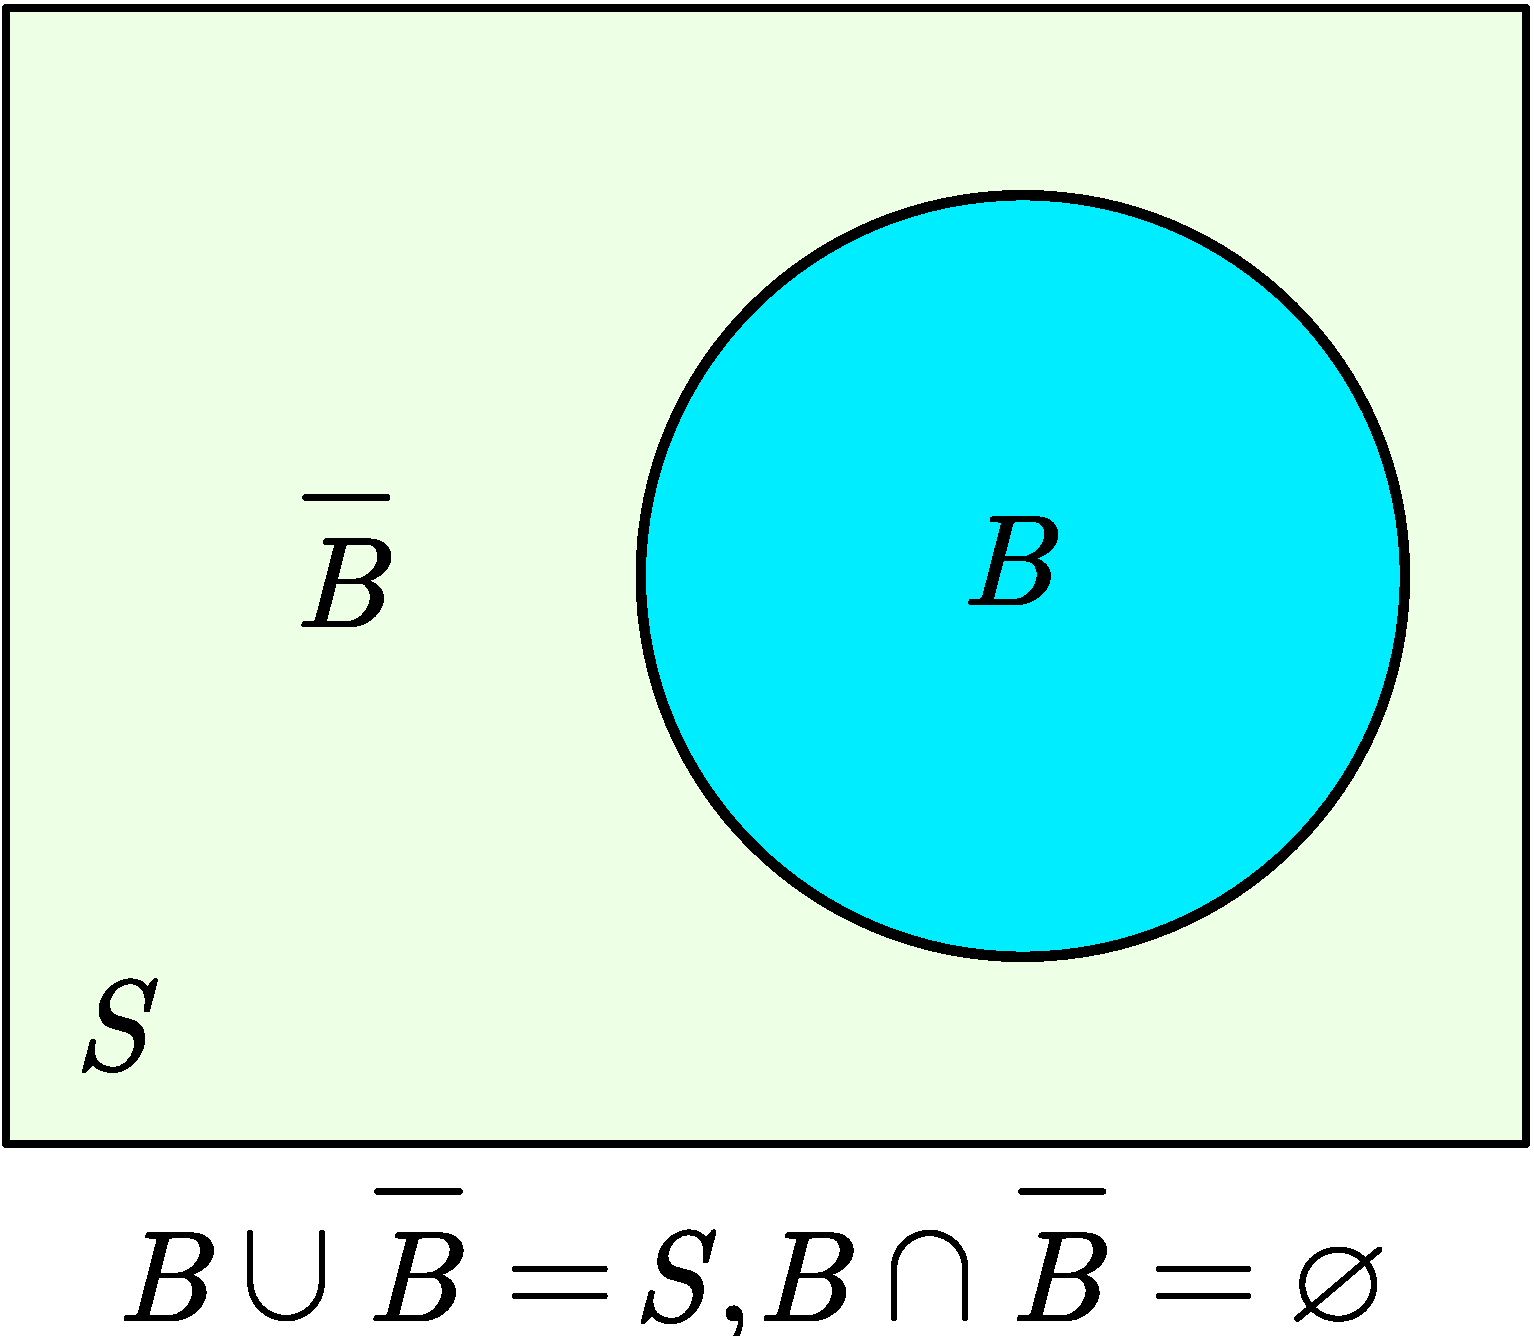
\includegraphics[width=0.8\linewidth]{sj6.pdf}
        \end{minipage}}
    \caption{事件间的关系韦恩图}
\end{figure}
设试验$ E $的样本空间为$ S $,而$ A,B,A_k(k=1,2, \cdots) $是$ S $的子集,则有:
\begin{enumerate}
    \item \nomenclature{$ A\subset B $}{事件$ B $包含事件$ A $}若$ A\subset B $,则称\textbf{事件$ B $包含事件$ A $}, \md{事件$ A $发生必导致事件$ B $发生}, \cf{sub-fig-1}.特别地,若$ A\subset B $且$ B\subset A $,即$ A=B $,则称事件$ A $与事件$ B $相等.
    \item \nomenclature{$ \a\cup\b $}{事件\a 与事件\b 的和事件}事件$ \a\cup\b=\{x\mid x\in\a\mbox{ or }x\in\b\} $称为事件\a 与事件\b 的\textbf{和事件}, \cf{sub-fig-2}. \md{当且仅当\a, \b 中至少有一件发生}时,事件$ \a\cup\b $发生.

          类似地,我们称$ \displaystyle\bigcup_{k=1}^nA_k $为$ n $个事件$ A_1,A_2, \cdots,A_n $的\md{和事件},称$ \displaystyle\bigcup_{k=1}^{\infty} A_k $为可列个事件件$ A_1,A_2, \cdots $的\md{和事件}.
    \item \nomenclature{$ \a\cap\b $, $ \a\b $}{事件\a 与事件\b 的积事件}事件$ \a\cap\b=\{x\mid x\in\a\mbox{ and }x\in\b \} $\margin{$ \a\cap\b $又记作$ \a\b $}称为事件\a 与事件\b 的\textbf{积事件}, \cf{sub-fig-3}. \md{当且仅当\a, \b 同时发生时},事件$ \a\cap\b $发生.

          类似地,我们称$ \displaystyle\bigcap_{k=1}^nA_k $为$ n $个事件$ \a_1, \a_2, \cdots, \a_n $的\md{积事件};称$ \displaystyle\bigcap_{k=1}^{\infty} A_k $为可列个事件件$ A_1,A_2, \cdots $的\md{积事件}.
    \item \nomenclature{$ A-B $, $ \a\backslash\b $}{事件\a 与事件\b 的差事件}事件$ \a-\b=\{x\mid x\in\a\mbox{ and }x\notin\b \} $称为事件\a 与事件\b 的\textbf{差事件}\margin{$ \a-\b $又记作$ \a\backslash\b $}, \cf{sub-fig-4}, \md{当且仅当\a 发生\b 不发生时},事件$ \a-\b $发生.
    \item \nomenclature{$ \a\cap\b=\varnothing $}{事件\a 与\b 互不相容(互斥)}若$ \a\cap\b=\varnothing $,则称事件\a 与\b \textbf{互不相容}的或\textbf{互斥}的, \cf{sub-fig-5}. \md{事件\a 与事件\b 不能同时发生}.基本事件是两两互不相容的.
    \item \nomenclature{$ \overline{A} $}{事件\a 的对立事件(逆事件)}若$ \a\cup\b=S $且$ \a\cap\b=\varnothing $,则称事件\a 与事件\b 互为\textbf{逆事件}或称\textbf{对立事件}, \cf{sub-fig-6}.这指的是对每次试验而言, \md{事件\a, \b 中必有一个发生,且仅有一个发生}. \a 的对立事件可以记为$ \overline{A} $且$  \overline{A}=S-A $.
\end{enumerate}


\begin{theorem}
    进行事件运算时我们常用到以下定律.设\a, \b, \c 为事件,则有
    \begin{enumerate}
        \item\textbf{交换律}:\begin{align*} \a\cup\b=\b\cup\a;\\\a\cap\b=\b\cap\a                                                              \end{align*}
        \item\textbf{结合律}:\begin{align*} \a\cup(\b\cup\c)=(\a\cup\b)\cup\c; \\ \a\cap(\b\cap\c)=(\a\cap\b)\cap\c .                                  \end{align*}
        \item\textbf{分配律}:若$ (\b\cup\c)\cap\a $发生,则\a 发生且\b 和\c 至少一个发生,则$ \a\cap\b $或$ \a\cap\c $发生.于是有\md{$ \a\cap(\b\cup\c)\subset(\a\cap\b)\cup(\a\cap\c) $}.反过来,若$ (\a\cap\b)\cup(\a\cap\c) $发生,则有$ \a\cap\b $或$ \a\cap\c $中至少有一个发生,从而$ \a\cap(\b\cup\c) $一定发生,由此可得\md{$ \a\cap(\b\cup\c)\supset(\a\cap\b)\cup(\a\cap\c), $}可得:\begin{align*} \a\cup(\b\cap\c)=(\a\cup\b)\cap(\a\cup\c); \\ \a\cap(\b\cup\c)=(\a\cap\b)\cup(\a\cap\c).             \end{align*}

        \item\textbf{德摩根律(对偶律)}:\margin{因为$ \overline{\a\cup\b} $表示\textquotedblleft\md{\a 和\b 中至少一个发生的否命题}\textquotedblright,即\md{\a 和\b 均不发生},由此可理解德摩根律.同时可以通过\textit{Fig \ref{sub-fig-2} }进一步理解与记忆\md{德摩根律}.}\begin{align*} \overline{\a\cup\b}=\overline{\a}\cap\overline{\b};  \\\overline{\a\cap\b}=\overline{\a}\cup\overline{\b}. \end{align*}
    \end{enumerate}
\end{theorem}

\section{频率与概率}
为了找到一个合适的数来表征事件在一次实验中发生的可能性大小,首先我们引入\md{频率},它描述了事件发生的\md{频繁程度},进而可以引出表征事件在一次试验中发生的可能性大小的数——\md{概率}.
\subsection{频率}
\definition[频率的定义]\label{def-frequency}
\margin{观察右式可知事件\a 发生的频率是它\md{发生的次数与试验次数之比}}在相同的条件下,进行了$ n $次试验,在这$ n $次试验中,事件\a 发生的次数$ n_A $称为事件\a 发生的\textbf{频数}.比值$ n_a/n $称为事件\a 发生的\textbf{频率},记作$ f_n(A) $,即有,其大小表示事件\md{发生的频繁程度},频率越大,事件\a 发生越频繁,在一次实验中发生的\md{可能性越大}.因而我们发现频率可以反应事件发生的可能性大小.\[ f_n(A)=\frac{n_A}{n} .\]

\begin{feature}[频率的性质]
    根据上述定义,不难发现以下性质:
    \begin{enumerate}
        \item $ 0\leqslant f_n(A)\leqslant 1 $;
        \item $ f_n(S)=1 $;
        \item 若$ A_1,A_2,\cdots,A_k $是\md{两两互不相容的事件},则\[ f_n\left(\bigcup_{i=1}^kA_i \right)=\sum_{i=1}^{k}f_n(A_i).  \]
    \end{enumerate}
\end{feature}

\subsection{概率}
大量试验证实,当重复试验的次数$ n $逐渐增大时,频率$ f_n(\a) $呈现出稳定性并逐渐稳定于某个常数.这种\md{频率稳定性}即所说的\textbf{统计规律性}.由于大量的试验成本巨大,为了理论研究的需要,我们从频率的稳定性与频率的性质得到启发,给出如下\md{能够表征事件发生可能性大小的概率的定义}.
\definition[概率的统计定义]
在对某一随机现象进行\md{大量的重复观测时},随着观测次数$ n $的增加,某一事件\a 的频率(\textit{cf. Def \ref{def-frequency}}):\[ f_n(A)=\frac{n_A}{n} \]会在某一个数$ p $(其中$ p\in[0,1] $)\md{附近摆动},我们称$ p $为事件\a 发生频率的稳定值.该值能够反应事件\a 发生的可能性大小,我们称之为\a 发生的\textbf{概率}.
\subsubsection{等可能概型(古典概型)}
\begin{definition}[古典概型]
    我们将具有以下特点:
    \begin{enumerate}
        \item 试验的样本元素只包含\md{有限个元素};
        \item 试验中每个基本事件发生的\md{可能性相同},
    \end{enumerate}的实验称为\textbf{等可能概型(古典概型)}
\end{definition}
\begin{definition}[概率的古典定义]
    设随机试验只有\margin{概率的古典定义是一种计算概率(等可能性)的数学模型,常称为\md{古典概型}.}$ \omega_1,\omega_2,\cdots,\omega_n $等$ n $个结果,每次实验\md{有且仅有其中的一个发生},并且每个结果\md{发生的可能性大小相同},我们可以定义事件\a 发生的概率为\[ P(A)=\frac{n_A}{n}, \]其中$ n_A $称为事件\a 包含于$ \left\lbrace \omega_1,\omega_2,\cdots,\omega_n\right\rbrace  $中元素的个数.
\end{definition}
\begin{theorem}[古典概型中事件$ A $的概率的计算方法]
    若事件$ A $包含$ k $个基本事件,即$ A=\{e_{i_1}\}\cup\{e_{i_2}\}\cup\cdots\cup\{e_{i_k}\} $,这里$ i_1,i_2, \cdots,i_k $是$ 1,2, \cdots,n $中某$ k $个不同的数,则有
    \begin{equation}\label{equ-gdgxjs}
        P(A)=\sum_{j=1}^{k}P(\{e_{i_j}\})=\frac{k}{n}=\frac{A\mbox{包含的基本事件数}}{S\mbox{中基本事件的总数}}.
    \end{equation}
    (\ref{equ-gdgxjs}) 式称为等可能概型中事件\a 的概率计算公式
\end{theorem}
\begin{example}[放回抽样与不放回抽样]
    已知袋中有$ a $只白球,$ b $只红球,$ k $个人依次在袋中取一只球分别作\textbf{放回抽样}和\textbf{不放回抽样},各求第$ i (i=1,2,\cdots,k)$人取到白球(事件\b)的概率.$ (k \leqslant a +b) $

    \textbf{解答:}	\begin{enumerate}[(1)]
        \item \textbf{放回抽样}: 每个人可能性显然相等,有\[ P(B)=\frac{a}{a+b}. \]
        \item \textbf{不放回抽样}:每个人各取一个球,每种取法是一个基本事件,共有\[\underbrace {(a + b)}_{{\footnotesize \mbox{\kaishu 第一个人}}}\underbrace {(a + b - 1)}_{{\footnotesize \mbox{\kaishu 第二个人}}} \cdots \underbrace {(a + b - k + 1)}_{{\footnotesize \mbox{\kaishu 第} k \mbox{\kaishu 个人}}} = A_{a + b}^k\]个基本事件.由\md{对称性}可知每个基本事件发生的可能性相同.当事件\b 发生时,第$ i $个人取的应是白球,它可能是$ a $中的某一只,所以有$ a $种取法.其余被取的$ k-1 $只球可以是其余的$ a+b-1 $只球中的任意$ k-1 $只\margin{此处只需要保证第$ i $个人取到白球(特定一个人取到白球),其他人任意取球即可.},共有\[ (a+b-1)(a+b-2)\cdots[a+b-1-(k-1)+1 ]=A^{k-1}_{a + b-1} \]种取法,于是事件\b 中包含$ a\cdot A^{k-1}_{a + b-1} $个基本事件,故由(\ref{equ-gdgxjs})式,可得\[ P(B)=a\cdot A^{k-1}_{a + b-1}/A_{a + b}^k=\frac{a}{a+b}. \]
    \end{enumerate}

    值得注意的是$ P(B) $与$ i $无关,即$ k $个人取球,尽管取球的先后顺序不一样,但计算发现,\md{每个人取到白球的概率一致},大家机会相同.此处可以可以提出一个有意思的理解方法,在后者未知前者取球结果的情况下,每人各自取球等同于随机分发,概率显然相等.若后者已知前者的取球结果,并且事件\b 已发生,那么后者取到白球的可能性下降,反之上升,由于前者的取球结果必然为白球或红球,即不能肯定前者取得的是白球(前者取到白球并非必然事件),那么对于后者来说这种可能上升可能下降的情况实际的总的取到白球概率仍然未变.这样亦可以解释到为何放回抽样与不放回抽样的概率结果相同.
\end{example}
\begin{example}[超几何分布]
    设有$ N $件产品,其中有$ D $件是次品,今从中任取$ n $件,问其中恰有$ k(k\leqslant D) $件次品的概率是多少?

    \textbf{解答:}在$ N $件产品中抽取$ n $件(不放回抽样),所有可能的取法共有$ \displaystyle\binom{N}{n} $
    \footnote{对于\md{任意实数}$ a $以及\md{非负整数}$ r $,定义\[ \binom{a}{r}=\frac{a(a-1)\cdots(a-r+1)}{r!}, \]特殊的,$\displaystyle \binom{a}{0}=1 $.当$ a $为\md{正整数},且$ r\leqslant a $时,$ \displaystyle\binom{a}{r} $即为组合数,即\[ \binom{a}{r}=\mathrm{C}^r_a\quad (r\leqslant a). \]}
    ,每一种取法为一基本事件,且由对称性知每个基本事件发生的可能性相同.又因在$ D $件次品中选取$ n $件,所有可能的取法有$ \displaystyle\binom{D}{k} $种.在$ N-D $件正品中取$ n-k $件所有可能的取法有$ \displaystyle\binom{N-D}{n-k} $种.有乘法原理知在$ N $件产品中取$ n $件,其中恰有$ k $件次品的取法共有$ \displaystyle\binom{D}{k}  \displaystyle\binom{N-D}{n-k}$种.于是所求概率为\begin{equation}\label{cjhfb}
        p=\frac{\displaystyle\binom{D}{k}  \displaystyle\binom{N-D}{n-k}}{\displaystyle\binom{N}{n}}.
    \end{equation}

    (\ref{cjhfb})式即\textbf{超几何分布}的概率公式.
\end{example}
\begin{example}[实际推断原理]
    某接待站在某一周曾接待过$ 12 $次来访,已知所有这$ 12 $次接待都是周二和周四进行的,问是否可以推断接待时间是有规定的.

    \textbf{解答:}假设接待站的接待时间没有规定,而各来访者在一周的任一天中去接待站是等可能的,那么发生如题所述事件的概率为:
    \[ p=\frac{2^{12}}{7^{12}}=0.000\ 000\ 3. \]可能性非常小,故接待时间应该是有规定的.\margin{根据\md{实际推断原理},现在概率很小的事件在一次试验中居然发生了,因此我们就有理由怀疑假设的正确性,从而推断出答案.}

    人们在长期的实践中总结到:
    \textbf{概率很小的事件在一次实验中实际上几乎不发生},我们称之为\textbf{实际推断原理}.
\end{example}
\subsubsection{几何概型}
\begin{definition}[概率的几何定义]
    设随机试验是往区域$ S $里投点,点落到$ S $中某子区域$ G $的可能性大小只与$ G $的度量大小有关,而与$ G $的形状和位置无关,则定义\[ P(\mbox{点落到子区域}G)=\frac{|G|}{|S|}, \]其中$ |\cdot| $表示几何度量,它可能是长度,面积等度量.

    我们称这种计算概率的数学模型为几何概型.
\end{definition}
\begin{example}[约会问题]
    两人相约在7点到8点间在某地会面,先到者可以等候20分钟,过时即离去.失球这两人会面的概率.

    \textbf{解答:}两人可能在区间$ [0,60] $的任一点到达,设$ x $和$ y $分别是两人到达的时间,则两人到达的时刻所对应的所有基本事件为二维区域$ D:[0,60]\rightarrow[0,60] $内的所有点,如图.而两人会面当且仅当\margin{
        \includegraphics[width=\marginparwidth]{cha1/jihedingyi.pdf}}\[ |x-y|\leqslant20, \]

\end{example}


\section{独立试验概型}

区别于事件独立性,我们可以提出试验独立的概念.
\definition[试验的独立性]
设有一组随机试验$  E_1,E_2, \cdots,E_n $.如果对$ E_i $的\md{任意结果(事件)}$ A_i $,都有\margin{事件独立和试验独立的区别, \md{事件独立}指的是\md{同一试验中的事件}, \md{试验独立}指的是\md{不同试验的事件}.}\[ P(A_1A_2\cdots A_n)=P(A_1)P(A_2)\cdots P(A_n), \]则称这组\textbf{随机试验相互独立}.










%打印索引—————————————
\newpage
\addcontentsline{toc}{chapter}{附录}
\addcontentsline{toc}{section}{索引}
\appendix
\kaishu
\color{titlepurple}
\printindex
%———————————————
\end{document}